%\begin{wrapfigure}{l}{8cm}
%	\centering
%		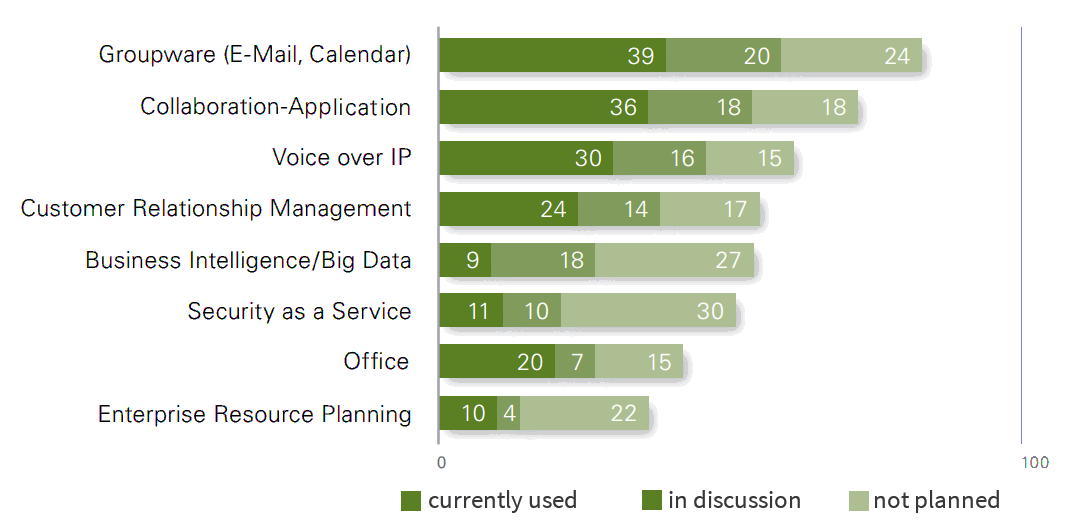
\includegraphics[width=0.75\textwidth]{images/cloud_application_germany.png}
%	\caption{CollaboraTeX form to import \LaTeX documents}
% \end{wrapfigure}

\chapter{Introduction}
Cloud Computing is a longstanding trend in Information Technology (\abk{IT}{Information Technology}) that quickly gained attention of decision makers and companies around the world once its full potential was realised. The key promisings of Cloud Computing are increased flexibility, better effectiveness of shared resources, less maintenance and significantly reduced costs.

It enables companies to outsource its technologies on different layers and migrate them to the services of Cloud providers. Today, \nameref{subsubsec:saas} is the most widespreach Cloud service, with 73\% of companies using it, followed by \nameref{subsubsec:iaas} with 47\% and \nameref{subsubsec:paas} with 33\%, according to a study by Gartner that consulted 2.300 Chief Information Officer (\abk{CIO}{Chief Information Officer}) worldwide \cite{website:gartner-cio-survey}.

Companies are increasingly relying on Cloud Computing and when considering the different \nameref{subsec:cloud-deployment-models}, there is clear evidence that hosting their private Cloud is equally important to them as the utilisation of other Cloud provider's services. At the same time, public services are much less common.

\begin{figure}[H] % \todo{vor Druck ändern -> h!}
	\centering
		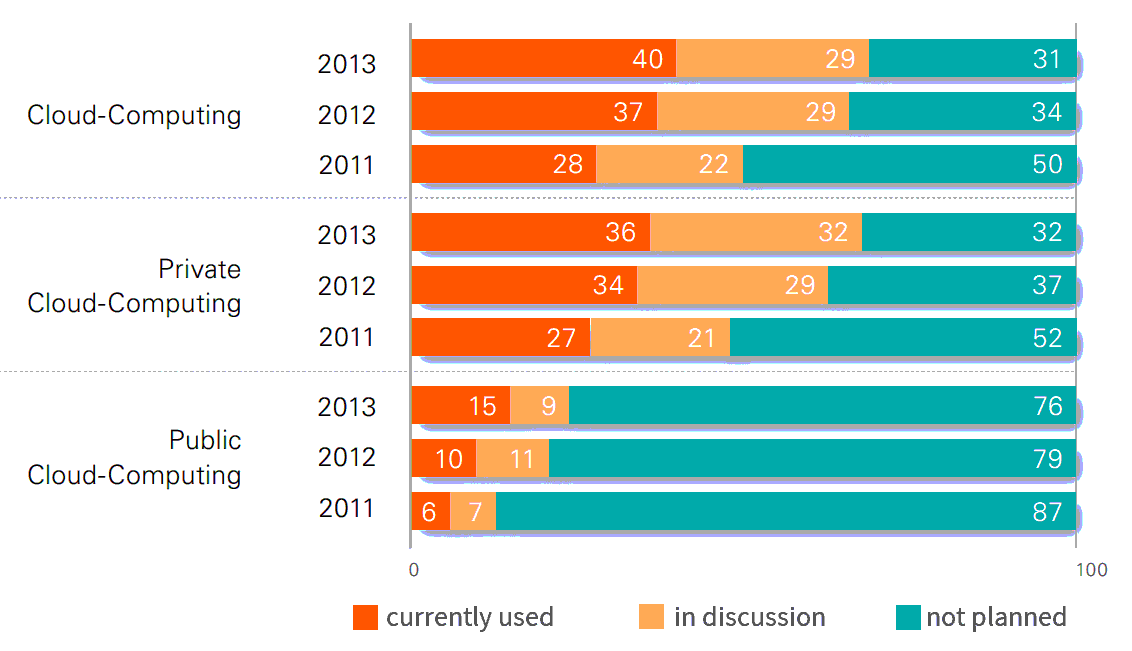
\includegraphics[width=0.8\textwidth]{images/cloud_usage_germany.png}
	\caption{Dominance of different Cloud \nameref{subsec:cloud-deployment-models} in the German market \cite{kpmg2014cloud}}
\end{figure}

As \nameref{subsubsec:saas} is the most important among all Cloud services for companies, the actual usage scenarios are regarded in the following. The most frequent form of using an application in the Cloud are groupware products, such as email and a calendar, followed by collaborative applications. More than half of all companies are currently utilising these tools.

The other two vital applications are Voice over IP and Customer Relation Management (\abk{CRM}{Customer Relation Management}) applications, while of the rest, Business Intelligence/Big Data, Security as a Service, Enterprise Resource Planning and Office, the latter is to be mentioned as still somewhat relevant.

\begin{figure}[H] % \todo{vor Druck ändern -> h!}
	\centering
		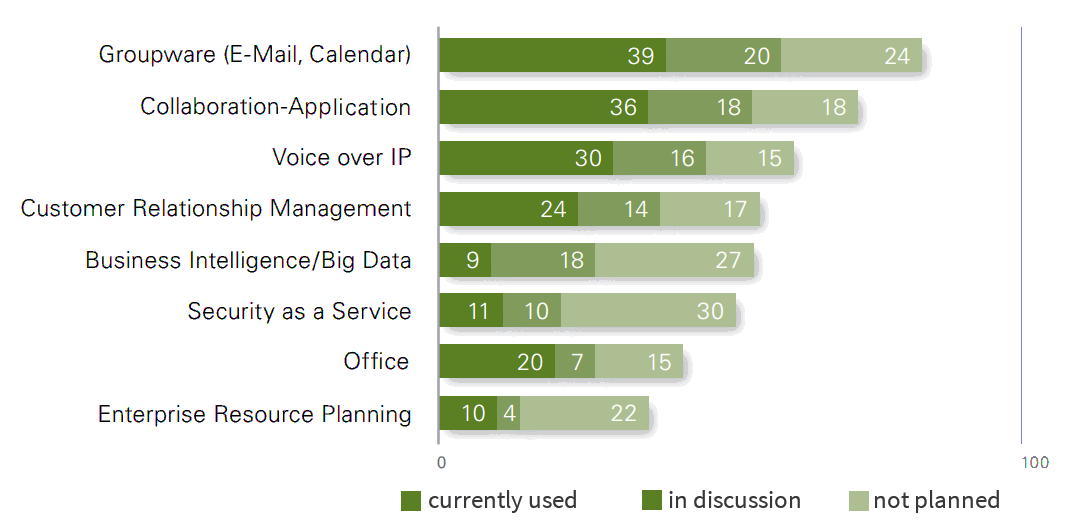
\includegraphics[width=0.85\textwidth]{images/cloud_application_germany.png}
	\caption{Different usage of \nameref{subsubsec:saas} in companies \cite{kpmg2014cloud}}
\end{figure}

And the majority of companies are quite satisfied with their experiences, 44\% of them perceive it as positive in every respect, 39\% as rather positive and only 17\% have a neutral opinion about their lessons learned.

However, as with everything in life, there is also a downside to the operation of Cloud Computing services and all its promises. In June 2013, it was revealed that the National Security Agency (\abk{NSA}{National Security Agency}) of the United States of America is wiretapping all major Internet companies with their top-secret \name{Prism} program \cite{website:guardian-prism}. It has been in operation since 2007 and is aimed to obtained direct access to the servers of Google, Facebook, Apple, Yahoo, Microsoft and others. 

This changed things on dramatic scale. It was previously known that American companies are legally obliged under US law to hand over data of their users, but the direct and unsupervised access of intelligence agencies to the companies' services is yet another dimension. It was disclosed by former employee Edward Joseph Snowden who cited the defence of information freedom as his main motivation \cite{website:guardian-snowden}.

Today it is known that the extent and nature of this surveillance by the NSA even exceeds the initial assumptions and there is even physical access to server hardware that it is being shipped by the manufacturer to its customer \cite{website:nsa-cisco}.

The teachings of this NSA scandal shaped the view of customers and companies for the Internet, its services and Cloud Computing. The confidence in the safety of data and the prevention of unauthorised access are nowadays the two major obstacles in companies to implement Cloud Computing services, stated by 57\% and respectively 71\% of all interviewed companies in Germany.

This shows immediate effect on the IT landscape, as half of the German companies already using or contemplating Cloud Computing are increasing their security requirements or even postponed or abandoned concrete projects.

\begin{figure}[H] % \todo{vor Druck ändern -> h!}
	\centering
		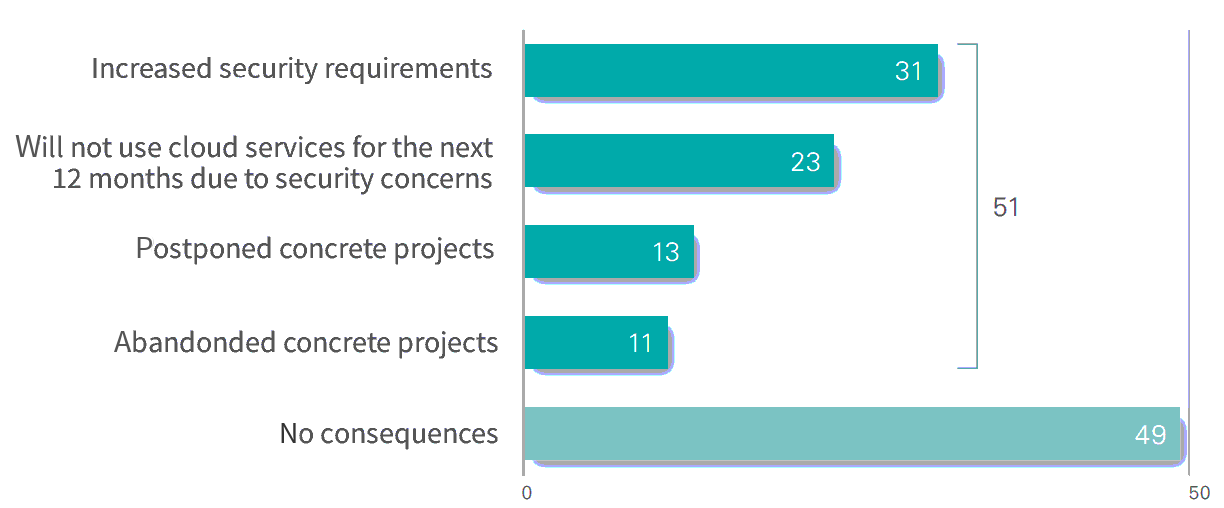
\includegraphics[width=0.9\textwidth]{images/cloud_nsa_consequences_germany.png}
	\caption{Consequences of the NSA scandal on the Cloud Computing strategies of German companies \cite{kpmg2014cloud}}
\end{figure}

It also makes politics appear on the scene. Revocation of the so-called \name{Safe Harbour Argreement}, that allows the legal transfer of individual-related data for European companies to the USA, was discussed by the European Parliament \cite{website:eupa-safe-harbour}. The NSA scandal and the teachings was also one of the major topics of the European elections in 2014. 

Simultaneously there are more and more potential security risks and sources of nonconformances are discovered, as the \name{Heartbleed} bug proved recently. It is a serious vulnerability in the OpenSSL cryptographic software library, which is prevalent on the Internet. The weakness allows the stealing of protected information that are usually encrypted by SSL/TLS and all major web server and operating systems are affected \cite{website:heartbleed}.

On the contrary, data are getting increasingly important for Internet companies, as the other new cool kid on the block besides Cloud Computing, \name{Big Data}, is another trend in IT. It underlines the old proverb \textit{"if you're not paying, you're the product"} as data embody a real business value for companies nowadays.

The numbers of companies and users with security concerns that scrutinise this business model however increases. Due to popular demand, private Cloud Computing is on the rise and ipso facto the premise of this work.

\pagebreak

\section{Scope and Aim}
\label{sec:scope-and-aim}

The idea to this work originates from two main factors. One of the major research areas of the Institute of Telematics (\abk{ITM}{Institute of Telematics}) of the University of Lübeck is Cloud Computing. It is this topic that the PhD thesis of Klaus-Dieter Schumacher focuses on: 

\begin{quote}
Forschungsgegenstand ist die Analyse der Möglichkeiten des Einsatzes von privaten Clouds im universitären Umfeld. Dabei soll auch untersucht werden, in welchem Umfang die in der Universität in den diversen Pools vorhandenen PCs für die Cloud genutzt werden können. Des Weiteren soll evaluiert werden, ob und in welchem Umfang im Rahmen einer Stiftungsuniversität Clouddienste anbietbar sind und durch dritte genutzt werden kann.

In einer ersten Testphase sollen ausgewählte Anwendungen implementiert und zunächst institutsintern angeboten und evaluliert werden.
\end{quote}

So on the one hand, a fully matured application that utilises the exisiting infrastucture is needed by the ITM. On the other hand, there is also a longstanding demand for a software that is capable of the collaborative editing of \LaTeX documents. With such an application it would be much easier for the staff to work on scientific research papers, academic exercises, exam papers and so on.

This leads eventually to the aim of this work: To develop a collaborative real-time \LaTeX editor that runs on the Cloud Computing infrastructure of the Institute of Telematics and provide the staff with the ability to work collaboratively on documents.

There was a exisiting solution to this problem, \name{\nameref{subsec:flylatex}}, but it was deemed as insufficient. However in the middle of this work, there was yet another, more mature application released as open source software, \name{\nameref{subsec:sharelatex}}, after already existing as closed source for several years. While it might have satisfied the requirements that were postulated by the members of the institute (compare chapter \ref{subsec:software-requirements}), it could not have been hosted the institute's existing infrastructure (compare chapter \ref{subsubsec:computing-resources}), therefore this work redevelops such a Software as a Service from scratch.

\section{Outline of this work}

This work is divided into five chapters. After the introduction into the topic, an explanation of the scope of this work will be given, followed by the overview of the conventions.

The second chapter will then illustrate the necessary theoretical foundations of \nameref{sec:cloud-computing} by illuminating its \nameref{subsec:cloud-history} and \nameref{subsec:cloud-standards} as well as \nameref{subsec:cloud-deployment-models} and \nameref{subsec:cloud-service-models}. Subsequently, \nameref{sec:collaborative-software} and its distinction to \nameref{subsec:collaborative-editing-foundations} will be reviewed and also the major algorithm behind it, \nameref{subsubsec:operational-transform}.

\pagebreak

In chapter three, existing online \LaTeX editors are reviewed and afterwards the \nameref{subsec:technical-constraints} and \nameref{subsec:software-requirements} elicited. Finally, the findings are analysed and presented.

The fourth chapter is dedicated to the \nameref{chap:architecture} resulting from this work. First of all, the \nameref{sec:approach-and-decision} is elucidated, before presenting the actual design in the respective subchapters Model, Services, Implementation and Tests.

The fifth and last chapter offers the conclusion of this work. It consists of an overlook of the \nameref{sec:implemented-functionalities}, succeeded by the consideration of possible following works and future additional implementations in the \nameref{sec:outlook}.

\section{Conventions}
As this work references various different technologies, applications, file formats, languages as well as classes, methods, packages and parameters, there are typographical conventions that will be followed thoughout this work.

\begin{table}[H]
	\begin{center}
		\setlength\extrarowheight{3pt}
		\begin{tabular}{ m{6cm} | m{3cm} }
		  	\textbf{Typographical Conventions} 	  & \textbf{Applies for} \\
			\hline                       
			\package{de.uniluebeck.package} 	  & Packages \\
			\class{Classname} 					  & Classes \\
			\method{Methodname} 				  & Methods \\ % (including such for the HTTP protocol) \\
			\parameter{Parametername} 			  & Parameters \\
			\parametertype{Parametertype} 		  & Parameter Type \\
			\parametertype{Mediatype} 		      & Media Type \\
			\fileformat{.abc}		   			  & File Formats \\
			\name{Name} 			  			  & Names \\
		\end{tabular}
		\caption{Typographical conventions of this work}
	\end{center}
\end{table}

This example shows how a REST service is specified: 

\restwithparam{description}{method}{url/\{urlParam\}}{ConsumeMediaType}{ProduceMediaType}{param}{paramType}{returnType}

\pagebreak

Source code examples are following the conventions of their respective language. For the programming language \name{Java}, the code conventions defined by Sun Microsystems and retained by Oracle, apply \cite{website:java-conventions}.

This work was developed under the agile process model, using Netbeans as \abk{IDE}{Integrated Development Environment} and the Java Development Kit in version 7, Update 51.
